\documentclass[crop,tikz,border=5mm]{standalone}% 'crop' is the default for v1.0, before it was 'preview'
\usepackage{pgfplots}

\usepgfplotslibrary{colorbrewer}
\usetikzlibrary{math}
\usetikzlibrary{calc}
\usetikzlibrary{positioning}

\begin{document}

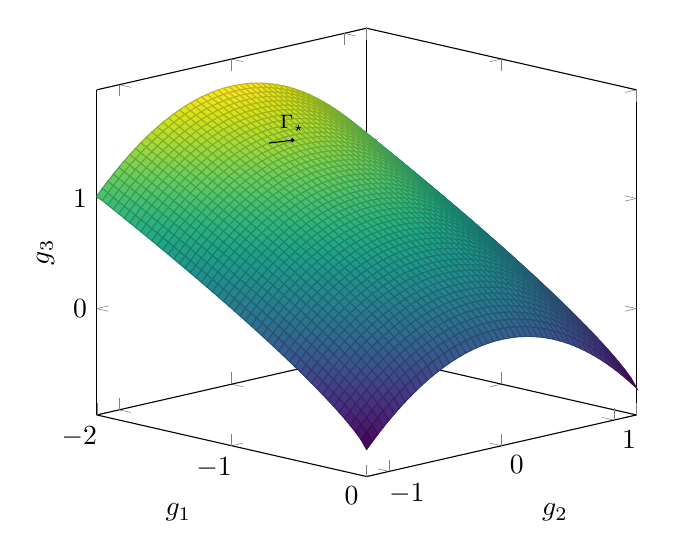
\begin{tikzpicture}[
  >=stealth,
  scale=1.00,
  ]

  % Coordinate system with UV critical surface
  \begin{axis}[
    % colormap name={RdBu-11},
    colormap/viridis,
    % colormap/PiYG,
    % shader=interp,
    view={45}{15},
    xlabel=$g_1$,
    ylabel=$g_2$,
    zlabel=$g_3$,
    % ticks=none,
    % xticklabels={,,},
    % yticklabels={,,},
    % zticklabels={,,},
    clip=false,
    ]

    \addplot3[
    surf,
    samples=50,
    domain=-2:0,
    y domain=-1.2:1.2,
    ] { abs(x)^(4/5) - y^2/2 };

    % Position of the points in theory space
    \addplot3[only marks, mark size=0.5pt] coordinates {(-1.55, 0, 1.375)};
    \node (P) at (axis cs:-1.55, 0, 1.37) [anchor=south] {$\scriptstyle \Gamma_\star$ };
    % \draw[->] (P) -- (axis cs-1.35, 0, 1.37);
    \addplot3[no marks] coordinates {(-1.55, 0, 1.375) (-1.60, -0.15, 1.37)};

  \end{axis}

\end{tikzpicture}

\end{document}
